\chapter{Linear Theory}

\section{Introduction and Motivation}
The stability of flows has a long and rich history within fluid dynamics. The classic experiment into the stability of fluid flow is that of  Reynolds \cite{reynolds1883}. In this experiment, Reynolds injected dye into the laminar flow through a pipe. By varying the velocity of the flow through the pipe. If the velocity was sufficiently low, Reynolds was able to observe ``a beautiful straight line through the tube". At slightly higher velocities, the straight line behaviour remained near the initial part of the pipe but further down ``the streak would shift about the tube, but there was no appearance of sinuosity". By increasing the velocity significantly, the dye would again initially remain straight near the initial part of the tube, but instead of shifting about the tube "the colour band would all at once mix up with the surrounding water, and fill the rest of the tube with a mass of coloured water". 

What Reynolds observed was the transition and breakdown of a flow into turbulence. Through careful observation, he determined that the dimensionless quantity that governed the behaviour of the flow was the Reynolds number 
\begin{align}
Re =\frac{UL}{\nu},
\end{align}
a number which, as discussed above represents the ratio between the inertial and viscous terms in the Navier-Stokes equations. Reynolds found that if $Re<13000$ then the flow would remain stable. The natural question to ask is to whether we can predict such numbers analytically or numerically. Due to the complex of the Navier-Stokes equations, a simplying approach must be derived. In order to do this, consider the following idea. Let $\bm{u}_{0}$ denote a basic state that solves the Navier-Stokes equations and let $\bm{u}'$ denote a small unknown perturbation such that $|\bm{u}'|\ll |\bm{u}_{0}|$. Mathematically this means
\begin{align}
\bm{u}(x,t) = \bm{u}_{0}(x,t) + \bm{u}'(x,t).\label{linear_def}
p(x,t) = p_{0}(x,t) + p'(x,t)
\end{align}
Now let us plug (\ref{linear_def}) into the Navier-Stokes equations and expand
\begin{align}
\frac{\partial \bm{u}_{0}}{\partial t} + \frac{\partial \bm{u}'}{\partial t} + (\bm{u}_{0}+\bm{u}')\cdot\nabla(\bm{u}_{0}+\bm{u}') = -\frac{1}{\rho_{0}}\nabla(p_{0} + p') + \nu\nabla^{2}(\bm{u}_{0} + \bm{u}')\\\label{expanded_lin_NS}
\nabla \cdot \bm{u}_{0} + \nabla \cdot \bm{u}'=0.
\end{align} 
Expanding out the advection term yields
\begin{align}
 (\bm{u}_{0}+\bm{u}')\cdot\nabla(\bm{u}_{0}+\bm{u}') &= \bm{u}_{0}\cdot\nabla\bm{u}_{0} + \bm{u}_{0}\cdot\nabla \bm{u}' + \bm{u}'\cdot\nabla\bm{u}_{0} + \bm{u}'\cdot\nabla\bm{u}'\\
&= \bm{u}_{0}\cdot\nabla\bm{u}_{0} + \bm{u}_{0}\cdot\nabla \bm{u}' + \bm{u}'\cdot\nabla\bm{u}_{0} + \mathcal{O}(\bm{u}'^{2})
\end{align}
where we have written the $\bm{u}'\cdot\nabla\bm{u}'$ term has $\mathcal{O}(\bm{u}'^{2})$ because this term is of order $\bm{u}'$ squared, which we assume to be small. Now recall that the basic state $\bm{u}_{0}$ solves the Navier-Stokes equations. Thus in (\ref{expanded_lin_NS}) there are terms that depend just on $\bm{u}_{0}$ and they will vanish by definition of it being a solution to the Navier-Stokes equations. Thus we now have that
\begin{align}
\frac{\partial \bm{u}'}{\partial t} + \bm{u}_{0}\cdot\nabla \bm{u}' + \bm{u}'\cdot\nabla\bm{u}_{0} + \mathcal{O}(\bm{u}'^{2})  = -\frac{1}{\rho_{0}}\nabla p' + \nu\nabla^{2}\bm{u}'\\
 \nabla \cdot \bm{u}'=0.
\end{align}
So far, the equation above is exact and we have just supressed the quadratic nonlinear term in the Big-O notation. Now the critical assumption we make is that because $\bm{u}'$ is small relative to the basic state, $\bm{u}'^{2}$ is even smaller thus is negligible. In other words, we are throwing away the quadratic nonlinearity of the perturbation term because it assumed to be small. 

This is an important point that can be sometimes lost in linear stability analysis. Since we are explicitly assuming that $|\bm{u}'|\ll |\bm{u}_{0}|$ the above equations are only valid when this is the case. As we shall see in numerical simulations, this assumption is not necessarily valid at all times. (Expand this a bit in terms of an energy discussion).

Now making the approximation that $\mathcal{O}(\bm{u}'^{2})$ is small we obtain
\begin{align}
\frac{\partial \bm{u}'}{\partial t} + \bm{u}_{0}\cdot\nabla \bm{u}' + \bm{u}'\cdot\nabla\bm{u}_{0} =  -\frac{1}{\rho_{0}}\nabla p' + \nu\nabla^{2}\bm{u}'\\
 \nabla \cdot \bm{u}'=0.
\end{align}
The above set of equations is linear which means they are more amenable to analytical techniques. 

To demonstrate an example of the general idea of linear stability, we will discuss the formulation of the experiment of Reynolds. This is a standard example and we follow the derivation of \cite{drazinreid}. It will also elucidate the key features of linear stability analysis that we will use below. 

The first simplifying assumption we make is that the basic state $\bm{u}_{0}=U(z)\hat{\bm{e}}_{x}$, a parallel shear flow, which simplifies the above equations to
\begin{align}
\frac{\partial \bm{u}'}{\partial t} + U\frac{\partial \bm{u}}{\partial x} + w'\frac{dU}{dz}\hat{\bm{e}}_{x}= -\frac{1}{\rho_{0}}\nabla p' + \nu\nabla^{2} \bm{u}'\\
\nabla \cdot\bm{u}'=0.
\end{align}
If we had considered the Euler equations instead of the Navier-Stokes equations, we would have the same equations as above except with $\nu=0$. Despite this seemingly simple modification, the resulting equation is very different. When the invsicid equations are considered, there are many elegant results that can be derived for the special case of parallel shear flow without specific what parallel shear flow we are considering. For example, the Rayleigh's inflection point theorem states that a necessary condition for instability is that the basic velocity profile should have an inflection pointer\cite{drazinreid}. A complete discussion of this result and others can be found in \cite{drazinreid,kundu}.

The next step is to expand the above solutions as Fourier modes (add more justification)
\begin{align}
\bm{u}'(x,t) = \hat{\bm{u}}(z)e^{i(\alpha x +\beta y -\alpha ct)}\\
p'(x,t) = \hat{p}(z)e^{i(\alpha x +\beta y -\alpha ct)}
\end{align}
where we take the real part of the above solutions. We require that the solution remainds bounded as $x,y\Rightarrow\pm\infty$ which means that $\alpha,\beta$ must remain real. For $c$, however, we let it remain an arbitrary complex number $c=c_{r} + ic_{i}$. Depending on the sign of $c_{i}$ the result will either decay or grown exponentially as time goes to infinity. We thus associate stability with $c_{i}\le 0$ and instability with $c_{i}>0$. Hence, if we are able to solve the above system and derive a criteria for the value of $c_{i}$ we will be able to derive some criteria for the stability of the flow.

Plugging in the above Fourier expansions into the linaer equations would yield an eigenvalue-eigenvector problem with $\alpha,\beta,c,Re$ being undetermined. From there we could apply numerical linear algebra routines to solve numerically for various $Re,\alpha,\beta$ and obtain a stability curve for $c$. However, a result due to Squire allows us to simplify the problem significantly. Squire's theorem states that to obtain the minimum critical Reynolds number it is sufficient to cosndier only two-dimesnional disturbances\cite{drazinreid}. In other words, for every three dimensional mode, there is a more unstable two dimensional eigenmode. A proof is provided in \cite{drazinreid}. 

Because we only need to consider two dimensional flow, the unknown velocity $\bm{u}'$ can be rewritten in terms of the stream function $\psi'(x,y,z,t)$. Another advantage of writing the equations in terms of the stream function is that the pressure is eliminated, as discussed in the previous sections, further reducing the number of unknowns. 

Denoting $\hat{\phi}$ as the amplitude of the stream function, the linear equations can be re-written as a single equation
\begin{align}
(D^{2}-\alpha^{2})^{2}\phi = (i\alpha \Re)(U-c)(D^{2}-\alpha^{2})\phi -(i\alpha \Re)U''\phi
\end{align}
along with the appropriate boundary conditions. This equation is known as the Orr-Sommerfeld equation and has a rich history in the development of fluid mechanics. A comprehensive review of the various methods of solving this equation, WKB theory, asymptotics, perturbation theory, and so, is contained in \cite{drazinreid} (van Dyke). 

This simple derivation has resulted in a single equation with three unknowns $\alpha,c,Re$ and by choosing different $Re$ and $\alpha$, we can determine a criteria for $c$. Although much work has been done at the beginning of the 20th century to derive approximate solutions to the Orr-Sommerfeld equation, numerically it is very easy to solve. We can reformulate the above equation as a generalised eigenvalue problem for a given parallel shear flow and solve the problem rather easily on a computer. (rewrite) (add Trefethen and some bits on how it relates Orr)

This example motivates the technique of linear stability. Here we have studied the Navier-Stokes equations directly instead of, the perhaps more promising, Euler equations. Recall the Euler equations arise by setting the viscosity to $0$ or letting the Reynolds number go to infinity. In the full blown problem of turbulence, a high Reynolds number on the order of $10^{8}-10^{9}$ is typical and since the inverse of the Reynolds number appears in front of the diffusion term, it seems reasonable to instead ignore the diffusion term since the coefficient is $\mathcal{O}(\Re^{-1}) \ll 1, Re\gg 1$. This would be a mistake. This is because the limit $Re\rightarrow\infty$ is a singular limit. Consider the following simplified model which arises in the study of boundary layers of shear bounded wall flow\cite{benderorszag,acheson_fluid,kundu}
\begin{align}
\epsilon y'' - y =0 \qquad y(0)=0,\qquad y(1)=1.
\end{align}
If we set $\epsilon=0$ we would obtain the equation 
\begin{align}
- y =0 \qquad y(0)=0,y(1)=1.
\end{align}
which clearly has no solution that satisfies the boundary conditions. If we tried a perturbation expansion of the form $y(x) =\sum_{n=0}y_{n}(x)\epsilon^{n}$ we would get nowhere because the lowest order term does not exist. If we solve the full equation, we see the problem with setting $\epsilon=0$,
\begin{align}
y(x) = \frac{e^{x/\epsilon}-1}{e^{1/\epsilon}-1}.
\end{align}
In this equation, we cannot set $\epsilon=0$ because that results in a singular limit. Thus regardless of how small we choose $\epsilon$, there will be a thin layer, called the boundary layer, which is essential to the fluid flow. For a discussion of techniques in singular perturbation theory in terms of the linear stability of the Navier-Stokes equations see \cite{drazinreid}.


\section{A Brief History of Vortex Instabilties}

The origin of vortex instabilities begins with Lord Kelvin who in 1880 studied perturbations to columnar vortices and determined that they were stable. For the next hundred or so years, the theory of vortex instability was quiet until the field was re-ignited by the investigations Crow\cite{crow1970}. Motivated by engineering applications, Crow was an aeronautical engineer, he discovered that for long wavelength perturbations of a pair of counter-rotating vortices that there was a symmetric deformation of the vortices. This worked extended a few years later by Widnall et. al \cite{widnall1974} to small wavelength perturbations. Further investigations into small wavelength perturbations were carried out by numerous others\cite{moore1975,tsai1976} (add in ref 3-7 bc1999) however these studies only considerd vortex filaments (define). It was noticed in these studies that the streamlines of the vortex became elliptical. Following through, Pierrehumbert\cite{pierrehumbert1986} investigated the simple case of a single 2D vortex subject to a constant 3D pertubation. Further work was done by Bayly \cite{bayly1986} and Waleffe\cite{waleffe1990}.

Something about the work of the japanese guys + experimental results. 

A complete and detailed history of the elliptical instability, including derivations and results of the above papers and nonlinear investigations, is presented in the review by Kerswell\cite{kerswell2002}.
\section{Zigzag Instability}
Motivated by the work above (cite), Billant and Chomaz investigate experimentally\cite{bc2000a}, theoretically\cite{bc2000b}, and numerically \cite{bc2000c} the evolution of a apair of columnar vortices in a stratified tank.

First Billant and Chomaz investigated the zigzag instability experimentally. To do this, they investigated a columnar vortex pair in a stratified fluid and investigated the evolution of the resulting flow. We now briefly discuss their experimental procedure since it provides important motivation for the resulting numerical study. 

In order to study the effects of stratification on the evolution of vortices, they first needs to create the vortices. To do this, they used a pair of motor-controlled flaps whose initial angle and closing time could be controlled precisely by a computer. When the flaps were closed, a pair of counter-rotating vortices was produced. They found that the important determining factor in the creation of the vortices was the angle of the flaps. If the angle was too small, additional vortices created when the flaps finally stopped closing were being advected by the dipole and causing spurious instability. For large angles fluid that was initially inbetween the flaps was being injected in the flow and again causing spurious oscillations. In order to balance out these effects, an angle of $14^{\circ}$ was chosen. After fixing the seperation angle they found that by varying the closing time of the flaps, the velocity of the pair of vortices could be changed. Interestingly, the decay of the vortices, roughly $90$s, was independent of the closing time of the flaps. This variation in the velocity determined the experimental parameters for the experiment.

The two important dimensional parameters in this experiment were the horizontal Froude number 
\begin{align}
F_{h} = \frac{U}{NR}
\end{align}
and the Reynolds numbers
\begin{align}
\Re= \frac{UR}{\nu}
\end{align}
where $U$ is the propagating velocity of the dipole as above, $R$ is the riadus of the dipole, $\nu$ is the viscosity of the tank, and $N$ is the buoyancy frequency. Here the viscosity $\nu$ and the radius $R$ were fixed by experimental conditions and could not be varied. Thus the only parameters that could be varied were $N$ and $U$. Since the Froude number was more difficult to vary, as changing it required draining and refilling the tank, the velocity was the only parameter that could be reasonably varied. Since $U$ shows up in both dimenionless numbers, changing $U$ resulted in the changing of both numbers, i.e. they are directly related by the following relationship
\begin{align}
\Re = F_{h}\frac{NR^{2}}{\nu}
\end{align}

To determine a theoretical model of the dipole, they computed the FFT of the measured vorticity in order to determine the streamfunction. They found that there was a linear fit between the vorticity $\omega$ and the streamfunction $\psi$ such that $\omega = -k^{2}\psi$ where $k^{2}=1.15$ which, as we will show below, corresponds to a Lamb-Chaplygin dipole. 

Add in result about using tape to excite most important mode and vertical orientation. 

A discussion of the theoretical paper will go here.

A discussion of the numerical paper will go here.


\section{Formulation of Problem}
We consider the non-dimensional Boussinesq approximation to the Navier-Stokes equations in Cartesian co-ordinates (ref from intro)
\begin{align}
\frac{D\bm{u}}{Dt} = -\nabla p - \rho'\hat{\bm{e}}_{z} + \frac{1}{Re}\nabla^{2} \bm{u},\\
\nabla \cdot \bm{u}=0,\\
\frac{D\rho'}{Dt} -\frac{w}{F_{h}^{2}} = \frac{1}{ReSc}\nabla^{2} \rho',
\end{align}
where $D/Dt=\partial/\partial t + \bm{u}\cdot \nabla, \bm{u}=(u,v,w)$ is the velocity, $p$ is the pressure, and $\rho'$ is the density perturbation. We have non-dimensionalised by the characteristic velocity $U$, length $R$, time-scale $R/U$, pressure $\rho_{0}U^{2}$, density $\rho_{0}U^{2}/gR$, and defined $Sc=\nu /D$ as the Schmidt number, where $D$ is the mass diffusivity, $\rho_{0}$ is the background density, and $g$ is the gravitational constant. The Reynolds and horizontal Froude number are as defined above. The buoyancy frequency $N$, and hence the Froude number $F_{h}$, is assumed to be constant. 

In order to investigate the linear growth rate, we proceed as the introduction and expand the full velocity field as the sum of a basic state and a perturbation state. 
\begin{align}
\bm{u} = \bm{u}_{0} + \tilde{\bm{u}}\\
p = p_{0} + \tilde{p}\\
\rho' = \rho'_{0} + \tilde{\rho}' 
\end{align}
here the basic state is the Lamb-Chaplygin dipole from above. 


\subsection{The Basic State} 
As the basic state for linear stability analysis we use the Lamb-Chaplygin dipole in a comoving frame \cite{meleshko1994}. This dipole is a solution to the 2D inviscid Euler equations. This basic state is motivated by numerous laboratory experiments\cite{bc2000a,leweke1998}, as discussed above, which demonstrated that a vertically oriented Lamb-Chaplygin dipole is a good approximation to the vortex generated by two flaps closing in a tank of salt-stratified water. The dipole, in cylindrical coordinates, is given by the stream function
\begin{align}
\psi_{0}(r,\theta) = 
\begin{dcases}
-\frac{2}{\mu_{1}J_{0}(\mu_{1})}J_{1}(\mu_{1}r)\sin\theta & r\le 1,\\\label{lc_dipole_sf}
-r\left(1-\frac{1}{r^{2}}\right)\sin\theta & r>1 ,
\end{dcases}
\end{align}
and the corresponding vertical vorticity $\omega_{z0}=\nabla_{h}^{2}\psi_{0}$
\begin{align}
\omega_{z0}(r,\theta) = \
\begin{dcases}
\mu_{1}^{2}\psi_{0}(r,\theta) & r\le 1,\\
0 & r>1,
\end{dcases}
\end{align}
where $J_{0},J_{1}$ are the zero and first order Bessel functions, $\mu_{1}\approx 3.38317$ is the first root of $J_{1}$, and $\nabla_{h}$ is the horizontal Laplacian. The basic state velocity is purely horizontal and is given by $\bm{u}_{h0}=\nabla_{h}\psi_{0}\times\hat{\bm{e}}_{z}$.

Let us now discuss the derivation of this result, which was first written down by Lamb and investigated further, independently, by Chaplygin. Although Lamb was the first to write down the above solution to the Euler equations, he did not provide any motiviation for the derivation beyond it being an exact solution of the 2D steady Euler equations. However, a decade later, Lamb provided a slightly more in depth derivation motivating somewhat the study of this dipole. Independently, in Russia, Chaplygin provided a complete derivation and motivation for studying this dipole, although it remained unknown outside of Russia. Following \cite{meleshko1994} we repeat the key points of Chaplygin's argument. 

Recall that the steady 2D Euler equations can be written in terms of the streamfunction $\psi$ and a vorticity $\omega$ as
\begin{align}
\nabla^{2} \psi = - \omega.\label{vort_eq_chap}
\end{align}
To choose $\omega$, Chaplygin was motivated by the situation where we have a continuous vortex whose outer region is steady irrotational flow while the inner region is a translating vortex. Recall that the potential function for a flow outside a cylinder is
\begin{align}
\psi = v_{0}\left(r - \frac{a^{2}}{r}\right)\sin\theta ,
\end{align}
where $a$ is the radius of the dipole and $v_{0}$ is the propogation velocity. 

Inside the radius $a$, Chaplygin chose the vorticity to be $\omega = n^{2}\psi$ where $n$ is a constant. In polar coordinates (\ref{vort_eq_chap}) becomes
\begin{align}
\frac{\partial^{2}\psi}{\partial r^{2}} + \frac{1}{r}\frac{\partial \psi}{\partial r} + \frac{1}{r^{2}}\frac{\partial^{2}\psi}{\partial \theta^{2}} =  n^{2}\psi
\end{align}
which we can guess at a solution of the form $\psi(r,\theta) = Z(r)\sin\theta$. Although Chaplygin did not provide specific motivation for choosing this specific vorticity, the above equation has a form that is similar to the irrotational flow outside the dipole and this makes the matching conditions simple. The resulting equation for $Z(r)$ is the well known Bessel equation (cite some book) and after grinding through the algebra, one obtains (\ref{lc_dipole_sf}). Chaplygin also investigated the resulting pressure field produced by the dipole and was able to compute the circulation of the dipole. Unlike Lamb, he also considered a generalisation of the above where the dipole is no longer symmetric about the x-axis. The corresponding vorticity in this case is given by
\begin{align}
\omega = n^{2}(\psi - \lambda)
\end{align}
where $\lambda$ is an arbitrary parameter where $\lambda=0$ is a completely symmetric dipole and $\lambda\rightarrow\infty$ corresponds to a completely asymmetric dipole. Here, again, Chaplygin investigated fully the pressure and circulation produced by this dipole. Additionally, in the same set of papers, Chaplygin also investigated the case of the dipole in rotating fluid, which was independently rediscovered 80 years later. Full details of this derivation are in \cite{meleshko1994} (flierl et. al) 

\subsection{Numerical Scheme}
We now write the fields as a basic state plus perturbations, denoted by $\sim$. Ignoring the viscous diffusion of the basic state \cite{drazinreid} (add tests from nonlinear code here to justify this point) and neglecting products of the perturbations, we obtain the following set of linear equations for the perturbations
\begin{align}
\frac{\partial \tilde{\bm{u}}}{\partial t} + \omega_{z0}\hat{\bm{e}}_{z}\times \tilde{\bm{u}}+\tilde{\boldsymbol{\omega}}\times \bm{u}_{h0} = -\nabla(\tilde{p}+\bm{u}_{h0} \cdot \tilde{\bm{u}}) - \tilde{\rho}'\hat{\bm{e}}_{z} + \frac{1}{Re}\nabla^{2}\tilde{\bm{u}},\label{nsl1}\\
\nabla\cdot\tilde{\bm{u}}=0,\\
\frac{\partial \tilde{\rho}'}{\partial t} + \bm{u}_{h0}\cdot \nabla_{h}\tilde{\rho}'-\frac{1}{F_{h}^{2}}\tilde{w} = \frac{1}{ScRe}\nabla^{2}\tilde{\rho}',\label{nsl3}
\end{align}
where $\tilde{\boldsymbol{\omega}}=\nabla \times \tilde{\bm{u}}$.

As stated above, the Lamb-Chaplygin dipole is oriented vertically. As a result we can separate the perturbation into the vertical and horizontal directions as 
\begin{align} 
[\tilde{\bm{u}},\tilde{p},\tilde{\rho}'](x,y,z,t) = [\bm{u},p,\rho'](x,y,t)e^{ik_{z}z} + \text{c.c.},
\end{align}
where c.c. is the complex conjugate. From here we can now take the 2D Fourier transform and and recall the projection operator $\textbf{P}(\textbf{k})$, with components $P_{ij}(\textbf{k})=\delta_{ij} - k_{i}k_{j}/k^{2}$ to eliminate pressure, to obtain a set of equations for the Fourier coefficients 
\begin{align}
\frac{\partial \hat{\bm{u}}}{\partial t} = \textbf{P}(\textbf{k})[\widehat{\bm{u}\times \omega_{z0}\hat{\bm{e}}_{z}} + \widehat{\bm{u}_{h0}\times\bm{\omega}}-\hat{\rho}'\hat{\bm{e}}_{z}] - \frac{k^{2}}{Re}\hat{\bm{u}},\label{solve1}\\
\frac{\partial\hat{\rho}'}{\partial t} = -i\bm{k}_{h}\cdot\widehat{\bm{u}_{h0}\rho'} + \frac{1}{F_{h}^{2}}\hat{w}- \frac{k^{2}}{ScRe}\hat{\rho}',\label{solve2}
\end{align}
where $k_{z},Re,Sc,F_{h}$ are input parameters, $\bm{k}_{h}=(k_{x},k_{y})$ is the horizontal wavenumber and $k^{2}=k_{x}^{2}+k_{y}^{2}+k_{z}^{2}$ is the total wavenumber. 

\subsection{Numerical Scheme}

To numerically solve (\ref{solve1}) and (\ref{solve2}), we use a spectral transform method to evaluate derivatives, with 2/3-rule de-aliasing and second order Adams-Bashforth for time-stepping. Each simulation was initialised with a random field and integrated over an $N\times N$ grid for 100 time units to determine the behaviour of the fastest growing mode. After several time units, the leading eigenmodes for $\bm{u},\rho$ behave exponentially (e.g. Billant and Chomaz \cite{bc2000c})
\begin{align}
\bm{u},\rho \propto C(x,y)e^{\sigma t},
\end{align}
and we can obtain the largest growth rate by the formula
\begin{align}
\sigma = \lim_{t\rightarrow\infty}\frac{1}{2}\frac{d\ln E}{dt}\label{sigma1},
\end{align}
where $\sigma$ is the real growth rate of the mode and $E$ is the kinetic energy $\frac{1}{2}(u^{2}+v^{2}+w^{2})$. This follows directly from the exponential behaviour of the leading eigenmode. The energy behaves as
\begin{align}
E \sim \frac{3}{2}C(x,y)^{2}e^{2\sigma t} \Rightarrow \ln E = \ln(3C^{2}/2) + 2\sigma t
\end{align}
and upon taking the time derivative of both sides yields the desired result. To obtain the energy, we use Parseval's theorem which relates the real space energy to the sum of the squares of the Fourier coefficients. Thus the total kinetic energy (domain averaged?) is obtained by summing the squares of the Fourier transform of the velocities over all wavenumbers. 

To evaluate $\sigma$, we compute the average value of the growth rate from the time series. Initially, there is transient behaviour where the various modes are all growing and none dominant (add figure of time series). After $t=20$, after the initial transient behaviour has died out and the leading mode dominants in all the cases observed. In the case of an oscillatory growth rate, as considered in \cite{bc1999}, we drop the assumption that $\sigma$ is real and instead compute the growth rate from
\begin{align}
\sigma_{r} = \lim_{t\rightarrow \infty} \frac{1}{2T}\ln\left(\frac{E(t+T)}{E(t)}\right)\label{sigma2},
\end{align}
where $T$ is the period of the oscillatory mode. (add figure of oscillatory growth rates). The imaginary growth rate is given as $\sigma_{i}=2\pi/T$. As above, we compute $\sigma$ from the time series beginning at $t=20$, however we first measure the period $T$ from roughly 10 oscillations, and then compute the average.  

For our simulations a grid size of $L=9$ with $N=512$ points was used with timestep $\Delta t=0.000950$ for $F_{h}=0.2,Re=2000,5000,10000$ and $\Delta t=0.000375$ for all the other simulations. Unlike Billant and Chomaz\cite{bc2000c} we did not restart each simulation with the previous eigenmode because we used a parallel approach for evaluating multiple $k_{z}$ simultaneously. We investigate a range of Froude and Reynolds number and a wide range of $k_{z}$ from $1$ to $200$ depending on the Froude and Reynolds number. This wavenumber range incorporates the scale of the zigzag instability down to the viscous damping scale. We take $Sc=1$ for all simulations.  

To simulate higher Reynolds number, we use a hyperviscosity operator. The $\nu\nabla^{2}$ diffusion term is replaced with a $\nu_{4}\nabla^{4}$ diffusion term. The $\nu_{4}$ coefficient is chosen so that $\nu k_{max}^{2} = \nu_{4}k_{max}^{4}$, where $k$ is the maximum dealiased horizontal wave number. This allows us to define the hyperviscosity Reynolds number $Re_{h}=Re k_{max}^{2}$. The hyperviscosity simulation was run with $F_{h}=0.1$ and $Re=20000$ with the same numerical parameters as the regular viscosity simulation.

\section{Results}

\subsection{Growth Rate}
Fig.~\ref{FixFhVaryRe} shows the largest eigenmode growth rate as a function of vertical wavenumber for fixed $F_{h}$ and $Re$. Following Billant and Chomaz\cite{bc2000c}, the scaled vertical wavenumber $k_{z}F_{h}$ is employed. The qualitative behaviour for the growth rates at different Reynolds numbers are very similar to one another. At small $k_{z}$, the growth rate reaches a local maximum, the zigzag peak, located at $k_{z}F_{h}\approx 0.6$ as predicted by Billant and Chomaz\cite{bc2000c}.  The growth rate then decreases for increasing $k_{z}$ to a local minimum before increasing to a second local maximum. Continuing to even smaller vertical scales, viscous effects increase and may damp out the instability, and hence the growth rate decays with increasing $k_{z}F_{h}$ in the limit of large $k_{z}F_{h}$. Oscillatory growth rates are observed for the smallest $k_{z}F_{h}$ as observed in Ref 26\nocite{bc1999}. The imaginary part of the growth rate $\sigma_{i}$ remains zero everywhere else except in a small region surrounding the local minimum between the zigzag and short-wave peaks. This oscillatory behaviour is not considered here. 

For $F_{h}=0.2$ (Fig.~\ref{FixFhVaryRe}a), the peak growth rate of the short-wave instability exceeds that of the zigzag instability for increasing Reynolds numbers. The growth rates at the second peak is smaller for $F_{h}=0.1$ (Fig.~\ref{FixFhVaryRe}b), but they continue to increase with increasing $Re$. For $F_{h}=0.05$ (Fig.~\ref{FixFhVaryRe}c), the second peak is weaker than the zigzag peak. Fig.~\ref{FixReVaryFh} shows the growth rate for fixed Reynolds numbers with varying Froude numbers. Examining the case of $Re=20000$ (Fig.~\ref{FixReVaryFh}a), the second peak increases with increasing Froude. A similar result is observed for $Re=10000$ and $5000$ (Fig.~\ref{FixReVaryFh}b-c). $Re=2000$ is not included because viscous effects have damped out the second peak in this case. Overall, the dependence of the short-wave growth rate on Froude is also more pronounced then that of Reynolds. For example, the growth rate of the second peak at fixed $Re=20000$ (Fig.~\ref{FixReVaryFh}a) doubles from $F_{h}=0.05$ to $F_{h}=0.2$. By contrast, at fixed $F_{h}=0.2$ (Fig.~\ref{FixFhVaryRe}a), the increase in the growth rate from $Re=5000$ to $Re=20000$ is only about $25\%$ larger. 

%\begin{figure}
%\begin{center}
%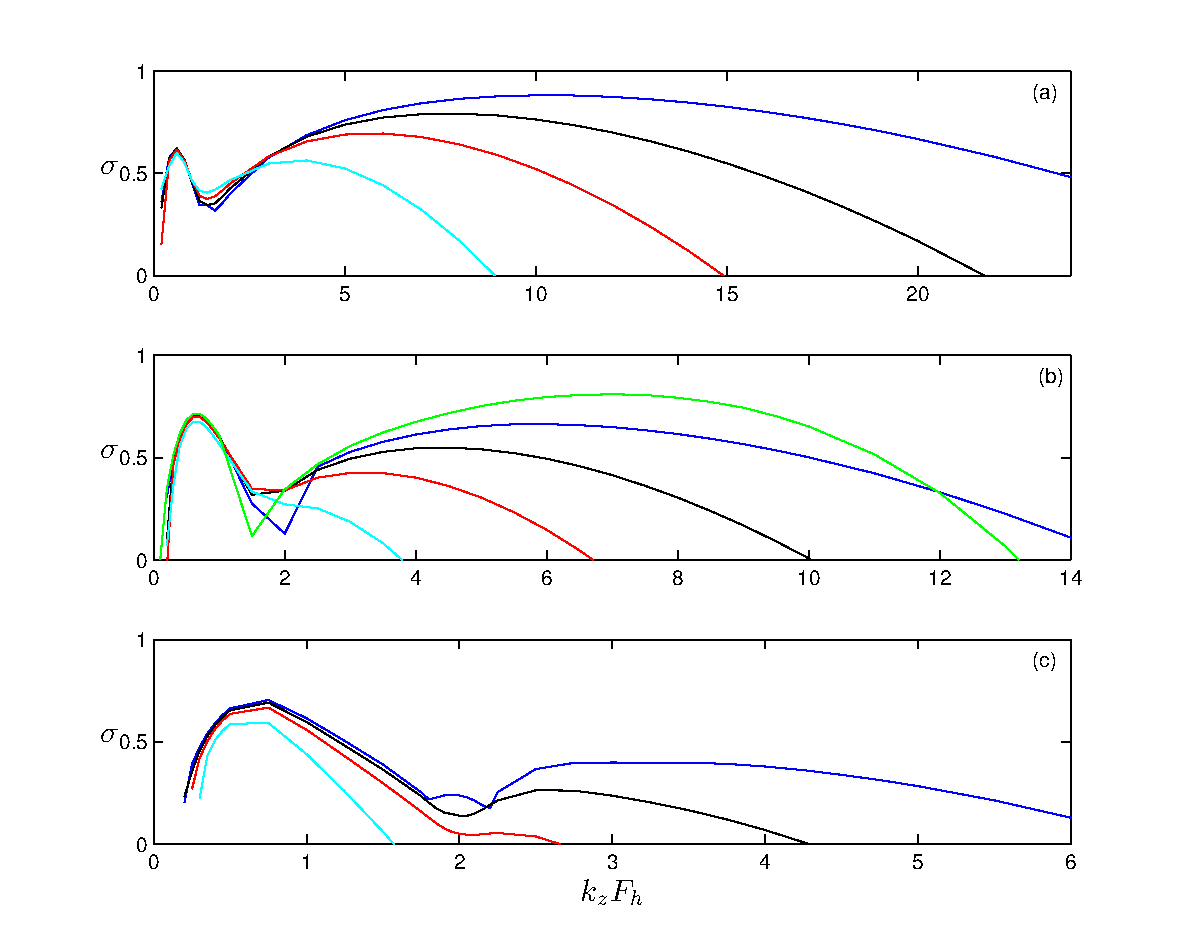
\includegraphics[width=\textwidth]{fixed_froude_varying_reynolds.eps}
%\caption{Growth rate $\sigma$ as a function of $k_{z}F_{h}$ for fixed $F_{h}=$(a) $0.2$, (b) $0.1$, (c) $0.05$ with Re$=2000$ (cyan), Re$=5000$ (red), Re$=10000$ (black), Re$=20000$ (blue). In panel (b) the green line is the hyperviscosity case with $Re=20000$.}
%\label{FixFhVaryRe}
%\end{center}
%\end{figure}
%\begin{figure}
%\begin{center}
%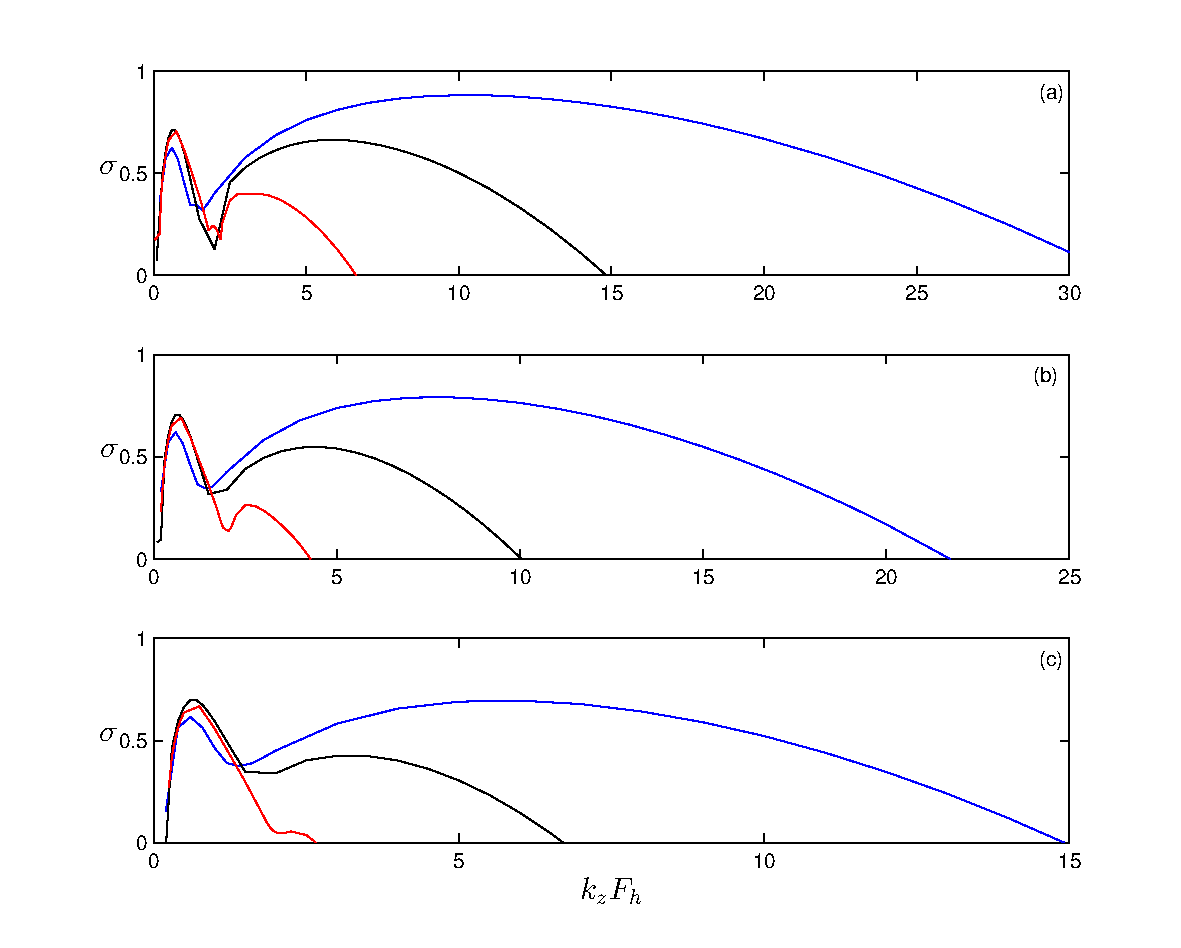
\includegraphics[width=\textwidth]{fixed_reynolds_varying_froude.eps}
%\caption{Growth rate $\sigma$ as a function of $k_{z}F_{h}$ for fixed $\text{Re}=(a) 20000, (b) 10000, (c) 5000$ with $F_{h}=0.05$ (red), $F_{h}=0.1$ (black), $F_{h}=0.2$ (blue).}
%\label{FixReVaryFh}
%\end{center}
%\end{figure}
The above analysis demonstrates that the short-wave growth-rate peak moves to larger $k_{z}F_{h}$ with increasing $F_{h}$ and increasing $Re$, but has a stronger dependence on Froude than Reynolds. Some of this joint dependence can be explained by examining the dependence on the buoyancy Reynolds number $Re_{b}=F_{h}^{2}Re$ \cite{riley2003,hebert2006,brethouwer2007}. In stratified turbulence, the buoyancy Reynolds number is analogous to the Reynolds number in the viscous term due to the vertical gradients \cite{brethouwer2007}. As $k_{z}$ increases, we move to smaller vertical scales where the vertical viscosity terms, controlled by the buoyancy Reynolds number, dominates, so it follows that the second peak may be governed by $Re_{b}$. In Fig.~\ref{Buoy} the location of the second peak from Fig.~\ref{FixFhVaryRe} is plotted as a function of the buoyancy Reynolds number. The peak location line is approximately linear and can be fitted with the curve $k_{z}F_{h}= Re_{b}^{2/5}$, which is plotted. This scaling implies that the vertical wavenumber, $k_{z}$, of the short-wave instability is approximately 
\begin{align}
k_{z} \sim F_{h}^{-1/5} Re^{2/5}\label{buoyscale}.
\end{align} 
The dependence of the growth rate on $k_{z}F_{h}$ appears to be similar in the cases with different $F_{h}$ and $Re$ but the same $Re_{b}$. Fig.~\ref{ReBuoy} demonstrates the similarity of the growth rate plotted against $k_{z}F_{h}$ for two cases with $Re_{b}=500$ and two cases with $Re_{b}=50$. For both cases, the locations of the zigzag and second peak line up quite well. The difference between the red and blue curves at the second peak is $4\%$ for $Re_{b}=200$ and $6\%$ for $Re_{b}=50$, a reasonable variation. 

% It is interesting to note that the red curve, corresponding to $Re=20000$ and $F_{h}=0.1$ (a), $F_{h}=0.05$ (b), is lower then the blue curve, corresponding to $Re=5000$ and $F_{h}=0.2$ (a), $F_{h}=0.1$ (b). This supports the observation, and is clear from the definition of the buoyancy Reynolds number, that the stratification may play a more important role in the instability than the viscosity.   

%\begin{figure}
%\begin{center}
%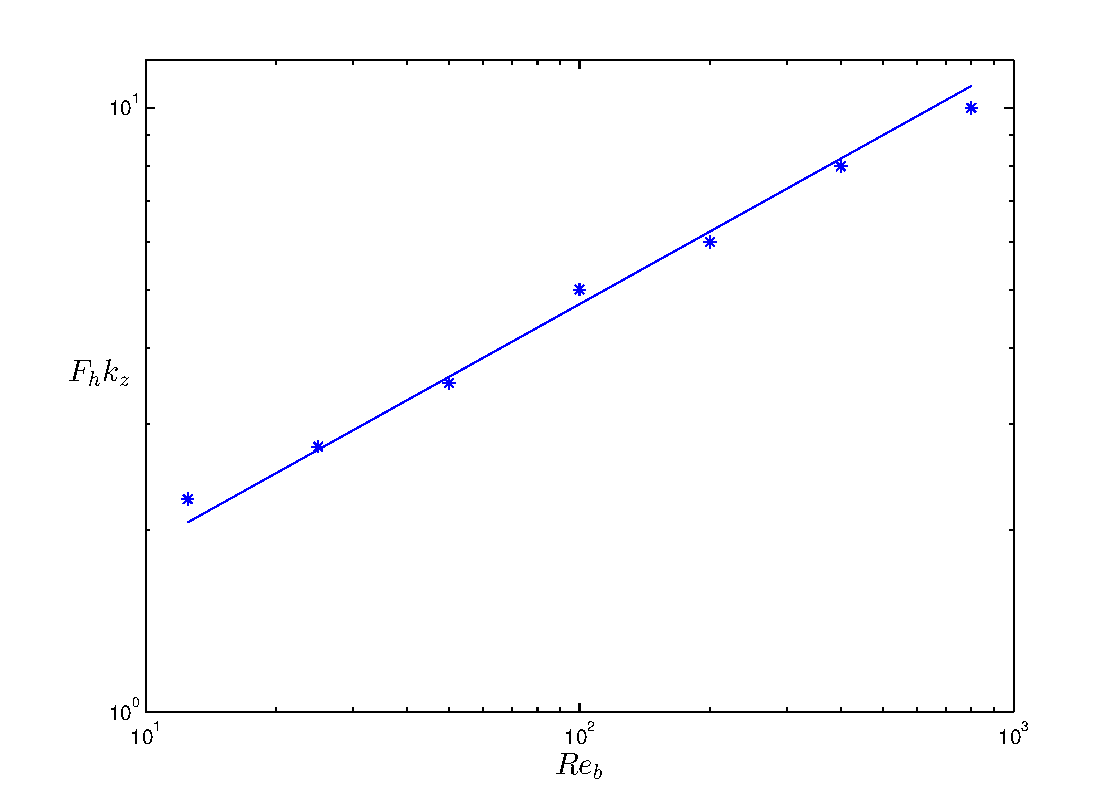
\includegraphics[scale=0.6]{second_peak_buoyancy.eps}
%\caption{The location of the second peak as a function of the buoyancy Reynolds number $Re_{b}$. $k_{z}F_{h}$ is taken from Fig.~\ref{FixFhVaryRe}. The straight line is $Re_{b}^{2/5}$.}
%\label{Buoy}
%\end{center}
%\end{figure}
%\begin{figure}
%\begin{center}
%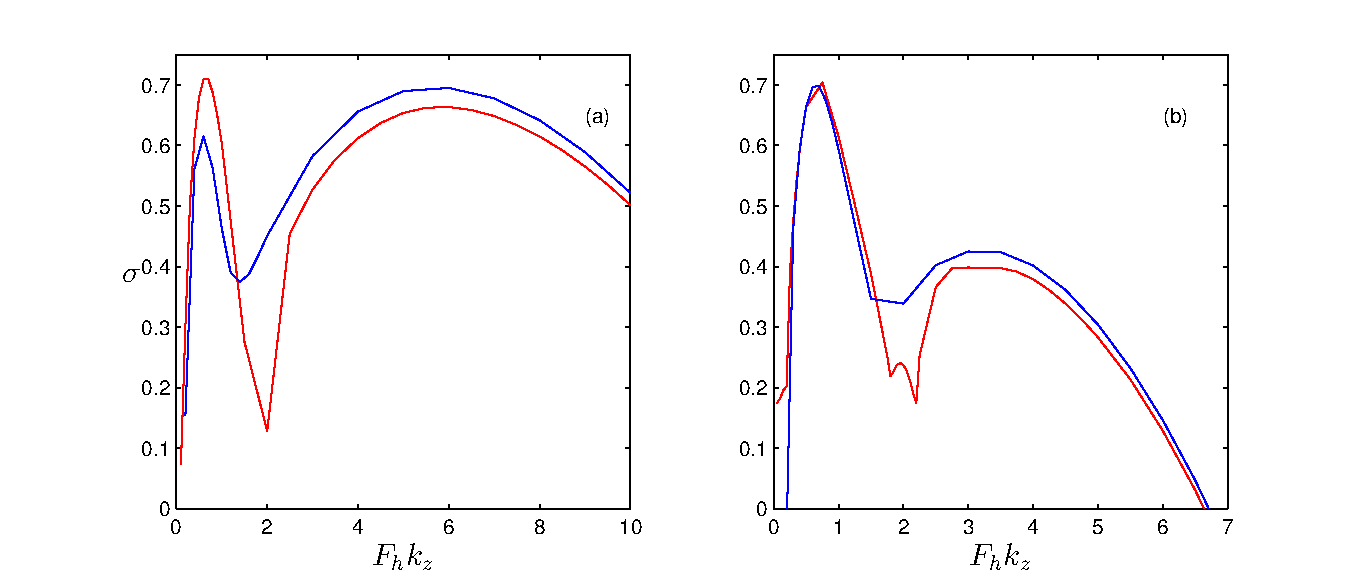
\includegraphics[width=\textwidth]{buoyancy_reynolds.eps}
%\caption{Growth rate $\sigma$ as a function of $F_{h}k_{z}$ for fixed $Re_{b}$. In (a), red is $Re=20000, F_{h}=0.1$ and blue is $Re=5000, F_{h}=0.2$, both corresponding to $Re_{b}=500$; in (b) red is $Re=20000, F_{h}=0.05$ and blue is $Re=5000, F_{h}=0.1$, both correpsonding to $Re_{b}=50$.}
%%\caption{Growth rate $\sigma$ as a function of $k_{z}$ for fixed $Re_{b}=(a) 200, (b) 50$. In (a) red corresponds to $Re=20000, F_{h}=0.1$ blue to $Re=5000, F_{h}=0.2$, in (b) red corresponds to $Re=20000, F_{h}=0.05$, blue $Re=5000, F_{h}=0.1$}
%\label{ReBuoy}
%\end{center}
%\end{figure}


In Fig.~\ref{FixFhVaryRe} (b) the green curve corresponds to a hyperviscosity run with $Re=20000$, which has $Re_{h}=2.8\times 10^{8}$. The motivation for using hyperviscosity is to capture higher-Reynolds number regime by restricting dissipation to only the largest wavenumbers. As the hyperviscosity run demonstrates, the zigzag peak is independent of Reynolds number and the existence of the peak would be expected at higher Reynolds numbers. For the second peak, we note that the growth rate  of the hyperviscosity run exceeds that of $Re=20000$ for $k_{z}F_{h}>3$ and reaches a maximum around $k_{z}F_{h}=7$. The maximum growth rate in the hyperviscosity case is around $25\%$ larger than the regular viscosity case with $Re=20000$. At $k_{z}F_{h}=12$ we see the hyperviscosity and non-hyperviscosity curves cross. This intersection corresponds to the horizontal wavenumber at which the hyperviscosity damping rate equals the regular viscous damping rate for $Re=20000$. For $k_{z}$ greater than this maximum, the hyperviscosity operator experiences greater damping than the regular viscosity, which can be seen by the sudden drop off of the growth rate. This simulation presents evidence that as $Re\rightarrow \infty$, the growth rate of the second peak will the same order as, or larger than, the growth rate of the zigzag instability. 

\subsection{Structure} 
%\begin{figure}
%\begin{center}
%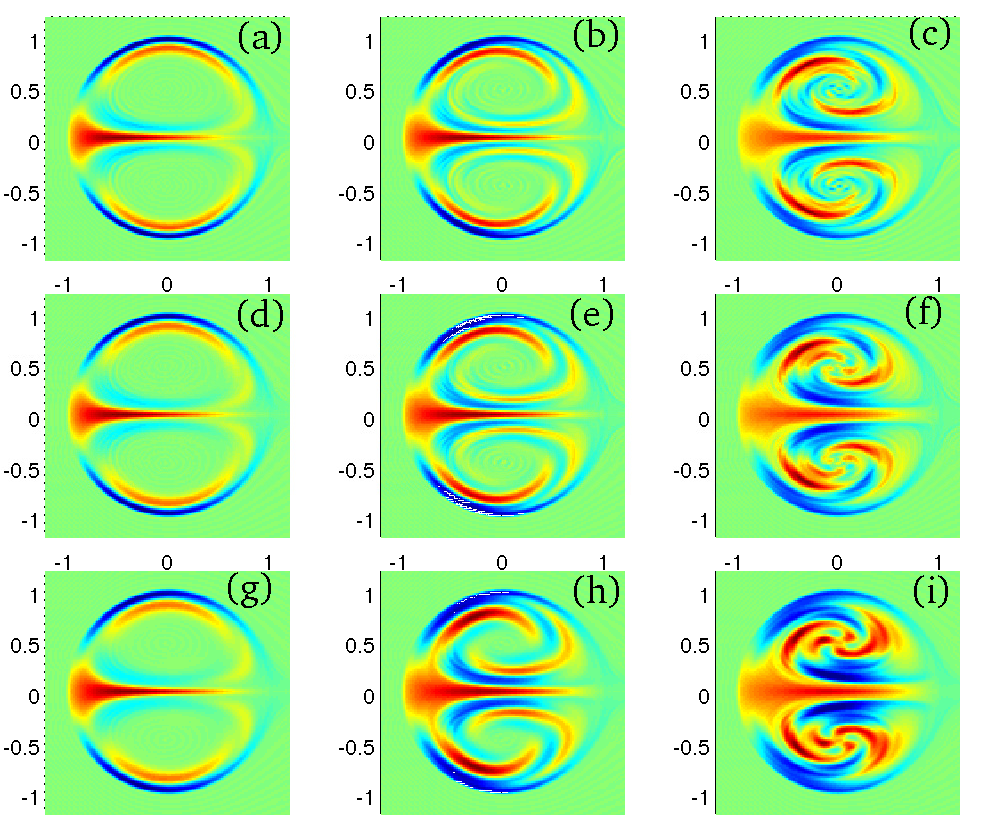
\includegraphics[width=\textwidth]{vorticity_second_peak.eps}
%%\caption{Perturbation vertical vorticity $\omega_{z}$ for $k_{z}$ at the second peak. $F_{h}=(a)(d)(g) 0.2 ,(b)(e)(h) 0.1, (c)(f)(i), 0.05, Re=(a)(b)(c) 20000, (d)(e)(f) 10000, (g)(h)(i) 5000$.}
%\caption{Perturbation vertical vorticity $\omega_{z}$ at second peak for $Re=20000\text{ (top) }, 10000 \text{ (middle) }, 5000 \text{ (bottom) }$; and $F_{h}=0.2 \text{ (left) }, 0.1 \text{ (middle) }, 0.05 \text{ (right) }$.}
%\label{secondpeak}
%\end{center}
%\end{figure}
Fig.~\ref{secondpeak} shows the spatial structure of the perturbation vertical vorticity at the second peak for different $Re$ and $F_{h}$. Qualitatively, we observe greater variation for different Froude numbers versus different Reynolds number as suggested above.  At the largest Froude number, the perturbation vorticity is organised in thin strips around and inside the dipole core between the two vortices. Panels (b),(e),(h) have $F_{h}=0.1$ and have a similar overall structure to the larger Froude number. Here, in the cores of the vortices, there is an emergence of a swirl-like pattern. At lower Reynolds number, the structure is spread out due to diffusion, while at higher Reynolds number, small-scale structure is beginning to emerge. This trend continues overall as we move to lower Froude numbers. 

Examining panels (g)-(i) (fixed $Re$ and decreasing $F_{h}$), the core of the dipoles has a twisting-like behaviour as the Froude number decreases. From this we can conclude that the instability structure of the second peak depends more on the Froude number than on the Reynolds number, which again reinforces the buoyancy Reynolds number scaling.  Indeed, if we consider the cases with $Re_{b}=50$ and $200$ as above, which correspond to Fig.~\ref{secondpeak} (b),(g) and (c),(h) respectively, we can see similar structure in the vorticity fields. Additionally, the anti-symmetric structure of the perturbation can be observed in the dominant eigenmodes in all cases, as found by Refs 17,26\nocite{bc1999,bc2000c}.

% The vorticity being very thin in the centre is consistent with the results of \cite{pierrehumbert1986} which examined unstratified inviscid vortices at small vertical scales which also demonstrated this behaviour. 
%\begin{figure}
%\begin{center}
%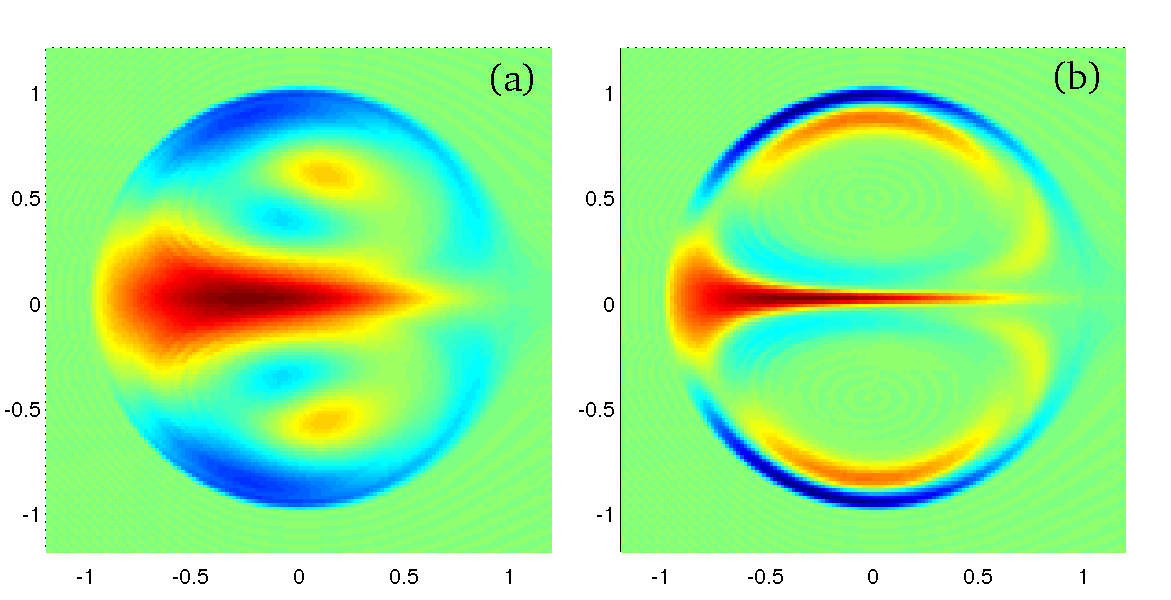
\includegraphics[scale=0.5]{second_peak_vs_zigzag.eps}
%\caption{Perturbed vertical vorticity $\omega_{z}$ at (a) the zigzag peak (b) the second peak for $Re=5000, F_{h}=0.2$}
%\label{zigzagcomparison}
%\end{center}
%\end{figure}

Fig.~\ref{zigzagcomparison} shows the perturbation structure for the zigzag peak (a) and the short-wave peak (b) for the case of $Re=5000,F_{h}=0.2$. This case was chosen because the growth rates of the two wavenumbers is roughly the same (see Fig~\ref{FixFhVaryRe} a). The zigzag instability exhibits a quadropole vorticity structure as discussed in Ref 17\nocite{bc2000c}, which corresponds to a bend and a twist of the basic state dipole. The short-wave instability shares some common overall structure with the zigzag instability. Both have a line of vorticity centred in between two Lamb-Chaplygin vortices and have a ring of vorticity negative vorticity around the outer edges of the dipoles. Additionally, the number of local maximum and minimum remains the same. However, in the short-wave instability, these bands of vorticity have been squeezed into thinner strips and are much more localised along the outer edges of the vortices. In the cores of the dipoles, there is almost no structure and we do not see a quadropole moment. The full vorticity field of the short-wave instability has a much more dominant twist then the zigzag instability and the bending of the dipole is reduced. As the stratification is increased, this behaviour continues but there is a significant emergence of structure within the cores of the vortices, as observed in Fig~\ref{secondpeak}.


\subsection{Subdominant modes?} 
The above analysis only provides the leading eigenvalue. Discuss subdominant mode ideas. Krylov method + matlab method.
\section{Dimensional Analysis}
That will go here. 


\section{Conclusion}

